% 03.12.2024: 645 Words - 7
%15 Min: 
%(1) 139 Words - 4
%(2) 315 - 2

% 10.12.2204: +1 +3 +1 +2

NLP is a subfield of AI that focuses on the interaction between computers and humans through natural language. LLMs are a type of Deep neural network models that has been trained on a large corpus of text data. They are predominantly based on the transformer architecture \cite{Wolf.09.10.2019}. 

\paragraph{Transformer Architecture}
There are many well-known models based on the transformer architecture, such as BERT, GPT-3.5, LLaMA, and others (\cite{Yin.2024}). The transformer architecture was introduced by Vaswani et al. in 2017. Briefly summarized it's based on the self-attention mechanism, which allows the model to weigh the importance of each word in a sentence. The architecture has been shown to outperform other architectures in various NLP tasks.

% include graphic of transformer architecture
\begin{figure}[h!]
    \centering
    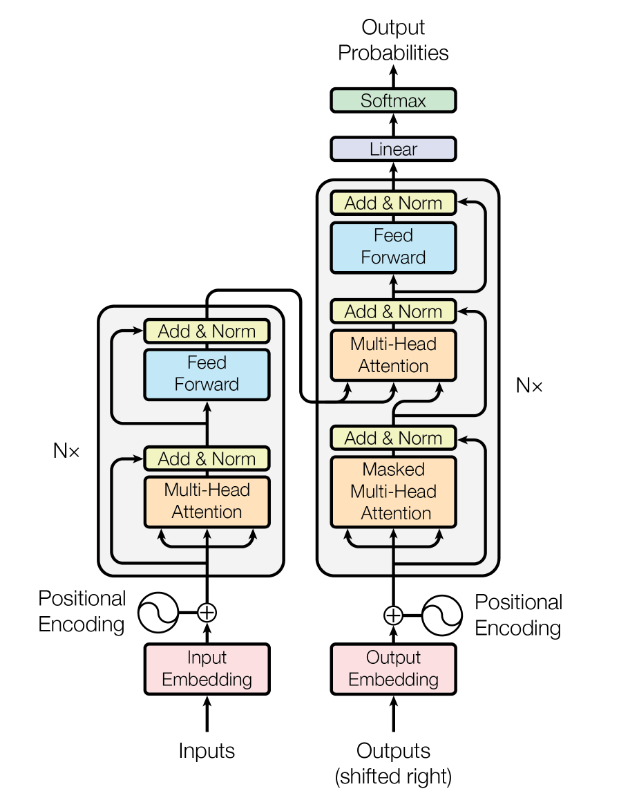
\includegraphics[width=0.6\textwidth]{images/transformers_architecture.png}
    \caption{Transformer Architecture, Source: \cite{vaswani2023attentionneed}}
    \label{fig:transformer_architecture}
\end{figure}

In the figure \ref{fig:transformer_architecture} the transformer architecture is shown. The encoder is processing the whole text. The decoder is autoregressive and uses its own outputs to generate further text. In the following the main components of the transformer architecture are explained.

\subparagraph{Encoder}

The encoder transforms the sequences in a list of tokens and passes them to the input embedding layer and to the the positional encoding layer. After that it gets passed to several layers of multi-head self-attention plus a feed forward neural network blocks. The outputs of the encoder is passed to the decoder, if the architecture is an encoder-decoder architecture. Encoders can also stand alone for tasks like text and code classification. (\cite{Hou.8212023})

\subparagraph{Decoder}

In the encoder-decoder architecture the decoder starts with an starting ouput sequence or an empty one. The output sequence is passed to the output embedding layer and to the positional encoding layer. After that it gets passed to several layers of masked and non-masked multi-head self-attention, plus a feed forward neural network blocks. The outputs of the decoder is passed to the output layer, which is a linear layer followed by a softmax function. The output layer predicts the next token in the output sequence. The output sequence is passed to the decoder again, so that the model can predict the next token based on the previous tokens. This process is called autoregressive generation.
The decoder can also stand alone for autoregressive tasks like code completion, text to code generation, debugging, etc. as shown in \cite{Hou.8212023}.

\subparagraph{Input Embedding}
Depending on the model, the input and output sequences are tokenized into subwords, words or characters. The input sequences are passed to the input embedding layer, which converts the tokens into a dense vector representation. The input embedding layer is trained along with the rest of the model. The output of the input embedding layer is passed to the positional encoding layer. The positional encoding layer adds information about the position of each token in the input sequence, so that the model can distinguish between words with the same token but different positions. The positional encoding layer is added to the input embedding layer before it is passed to the encoder. The output embedding is equivalent to the input embedding, but it is used to convert the output tokens into a dense vector representation. The output embedding is used in the decoder part of the transformer architecture.

\subparagraph{Multi-Head Self-Attention Block}

Both in the encoder and in the decoder, a block consists of several multi-head self-attention layers followed by a feed-forward neural network layer. The multi-head self-attention layer is the main component of the transformer architecture. It allows the model to weigh the importance of each token in the input sequence for each other token. The multi-head self-attention layer consists of multiple heads. Each head consists of a Query, Key and Value matrix, which are used to calculate the attention scores between the input tokens. The attention scores are used to weigh the importance of each token in the input sequence for each other token. The formula is given by:

$$Attention(Q,K, V) = softmax(\frac{QK^T}{\sqrt{d_k}})V$$

Query (Q), Key (K) and Value (V) are matrices of the input tokens. This mechanism is based on common retrieval. Query can be seen as the search query, Key as the potential candidates and Value as the retrieved information.

All matrices are learned during training. Query and Key are used to calculate the attention scores. The division by $\sqrt{d_k}$ is used to stabilize the gradients during training. The softmax function is used to normalize the attention scores. For the decoder part with the masked multi-head self-attention, the attention scores are masked with $-\infty$ for every token after the current calculated one right before the softmax, so that the model can only attend to previous tokens in the output sequence and the next predicted token is based only on the previous tokens. All heads are gonna sumed up and passed through a linear layer, which is finally followed by a layer normalization to stabilize the gradients during training. 

\subparagraph{Putting it all together}
After the input sequence is passed through the encoder, the output sequence is passed through the decoder. The decoder uses the encoder output as additional input and autoregressively predicts the next token in the output sequence. The output sequence is passed to the output layer, which is a linear layer followed by a softmax function. The output layer predicts the next token in the output sequence. The output sequence is passed to the decoder again, so that the model can predict the next token based on the previous tokens. This process is called autoregressive generation.

There are several ways to predict the next token within the output layer. The most straightforward way is to predict the token with the highest probability. This is called greedy decoding. Another way is to sample the next token from the probability distribution. This is called sampling. There are also other ways to predict the next token, such as beam search, nucleus sampling, top-k sampling, top-p sampling, etc. These methods are used to improve the performance of the model. In the following the most important tuning parameters for LLMs are explained.

\section{Important Tuning Parameters for LLMs}

There are several tuning parameters that can be used to improve the performance of LLMs. Some of the most important tuning parameters are:

\paragraph{Temperature}
The temperature parameter is used to control the randomness of the generated text. A high temperature value leads to more randomness, while a low temperature value leads to less randomness. The temperature parameter T is added in the softmax function:

%include graphic
\begin{figure}[h!]
    \centering
    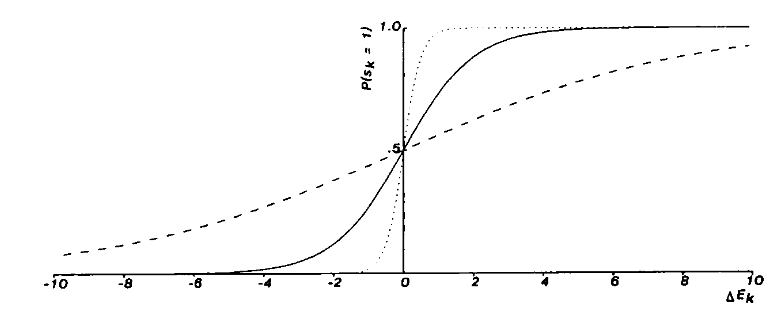
\includegraphics[width=0.6\textwidth]{images/temperature.png}
    \caption{The softmax function with different temperature values, T=1.0 (solid), T=4.0 (dashed), T=0.25 (dotted), Source: \cite{ACKLEY.1985}}
    \label{fig:temperature}
\end{figure}

$$softmax: o(z)_i = \frac{e^{\beta z_i}}{\sum_{j=1}^K e^{\beta z_i}}$$

In figure \ref{fig:temperature} the softmax function is shown. A low temperature value leads to a peaky distribution, while a high temperature value leads to a more uniform distribution and therefore to more randomness.


% split paragraph in two parts
\paragraph{Top-K Sampling}
Top-K sampling by \cite{Fan.13.05.2018} samples from the top K tokens with the highest probability before applying the softmax function. Therefore the higher the K value, the more tokens are considered for sampling. The outcomes gets more random. With Top-K equal to 1, the model behaves like greedy decoding.

\paragraph{Top-P Sampling}
The Top-P sampling by \cite{Holtzman.22.04.2019} samples from the smallest set of tokens whose cumulative probability exceeds the probability P. Therefore the higher the P value, the more tokens are considered for sampling. The outcomes gets more random. It is a generalization of Top-K sampling, where the number of tokens to sample from is not fixed.